% !TEX program = pdflatex
% Supplemental Material for the PRL-format theory draft.
\documentclass[aps,prl,reprint,superscriptaddress,nofootinbib,floatfix]{revtex4-2}

\usepackage[T1]{fontenc}
\usepackage{lmodern}
\usepackage{microtype}
\usepackage{amsmath,amssymb,bm}
\usepackage{graphicx}
\usepackage{booktabs}
\usepackage[hidelinks]{hyperref}

\hypersetup{
  pdftitle={Supplemental Material: double radiation cancellation at an acoustic Rayleigh threshold},
  pdfauthor={Author names to be inserted}
}

\newcommand{\ii}{\mathrm{i}}
\newcommand{\e}{\mathrm{e}}
\providecommand{\hom}{\mathrm{hom}}
\providecommand{\dr}{\mathrm{dr}}

\renewcommand{\theequation}{S\arabic{equation}}
\renewcommand{\thetable}{S\arabic{table}}
\renewcommand{\thefigure}{S\arabic{figure}}

\begin{document}

\title{Supplemental Material for ``Double Radiation Cancellation at an Acoustic Rayleigh Threshold''}
\author{Author Name}
\affiliation{Affiliation to be inserted}
\author{Coauthor Name}
\affiliation{Affiliation to be inserted}
\date{\today}
\maketitle

\section{Scope, conventions, and reproducibility}

The main Letter reports a theory result for an infinite, rigid, lossless
periodic surface.  This Supplemental Material gives the modal-matching
operator, the strict Rayleigh criterion, numerical convergence, complex-pole
tracking, field normalization, cavity ablation, dimensional scaling,
fabrication perturbations, and driven-scattering controls.  The final retained
design is evaluated at $f_0=200$~kHz and $c_0=1500$~m/s.  Pressure has time
dependence $\e^{+\ii\omega t}$; reflected propagating waves and evanescent
waves use the outgoing/decaying square-root branch.  Superscripts $\hom$ and
$\dr$ distinguish homogeneous eigenmode amplitudes from driven scattering
amplitudes.

The strict result uses $(N,K)=(313,39)$, where $N$ is the odd number of
Floquet orders and $K$ is the number of cosine modes per groove.  The final
same-geometry pole uses the same truncation.  Separate lower- and higher-order
calculations state their truncations explicitly.  All numerical figures are
generated from machine-readable MAT/CSV files.  The figure drivers are listed
in the data-and-code map below.

\section{Modal matching}

For a period $a$, incidence angle $\theta$, and $k_0=\omega/c$,
\begin{equation}
 k_{x,n}=k_0\sin\theta+\frac{2\pi n}{a},\qquad
 k_{y,n}=\sqrt{k_0^2-k_{x,n}^2},                                      \label{eq:s-k}
\end{equation}
where $\Re k_{y,n}\geq0$ and $\Im k_{y,n}\leq0$.  With the surface at
$y=0$ and water in $y>0$,
\begin{equation}
 p_{\mathrm{inc}}=\e^{-\ii k_{x,0}x+\ii k_{y,0}y},\qquad
 p_{\mathrm{sc}}=\sum_n A_n^{\dr}
 \e^{-\ii k_{x,n}x-\ii k_{y,n}y}.                                    \label{eq:s-exterior}
\end{equation}
The normalized variables are
\begin{equation}
 \Omega=\frac{af}{c},\qquad \kappa=\Omega\sin\theta,\qquad
 |\kappa+n|=\Omega                                                    \label{eq:s-ra}
\end{equation}
at the Rayleigh opening of order $n$.

Groove $\ell$ occupies $x_\ell<x<x_\ell+w_\ell$ and
$-d_\ell<y<0$.  The bottom-rigid expansion is
\begin{equation}
 p_\ell(x,y)=\sum_{q=0}^{K-1}C_{\ell q}
 \cos\!\left[\frac{q\pi(x-x_\ell)}{w_\ell}\right]
 \cos[\beta_{\ell q}(y+d_\ell)],                                    \label{eq:s-groove}
\end{equation}
\begin{equation}
 \beta_{\ell q}^2=k_0^2-\left(\frac{q\pi}{w_\ell}\right)^2.          \label{eq:s-beta}
\end{equation}
The pressure projection used in the code is
\begin{equation}
 \Pi_{n,\ell q}=\frac{1}{w_\ell}
 \int_{x_\ell}^{x_\ell+w_\ell}
 \e^{-\ii k_{x,n}x}
 \cos\!\left[\frac{q\pi(x-x_\ell)}{w_\ell}\right]\mathrm{d}x.      \label{eq:s-proj}
\end{equation}
Cosine norms are $1$ for $q=0$ and $1/2$ for $q>0$.

Let $\mathsf B$ map exterior pressure amplitudes to aperture cosine tests,
and let $\mathsf D$ map groove normal velocity to global Floquet tests.  With
\begin{align}
 \mathsf C_d&=\operatorname{diag}[\cos(\beta_{\ell q}d_\ell)],\nonumber\\
 \mathsf V_d&=\operatorname{diag}[(\beta_{\ell q}/k_0)
 \sin(\beta_{\ell q}d_\ell)].                                      \label{eq:s-cv}
\end{align}
the pole-free homogeneous operator is
\begin{equation}
 \mathsf F
 \begin{bmatrix}\bm A^{\hom}\\ \bm C\end{bmatrix}=0,
 \qquad
 \mathsf F=
 \begin{bmatrix}
   \mathsf B&-\mathsf C_d\\
   \operatorname{diag}(k_{y,n}/k_0)&\ii\mathsf D\mathsf V_d
 \end{bmatrix}.                                                       \label{eq:s-block}
\end{equation}
The $C_{\ell q}$ are retained as unknowns.  This avoids the tangent poles
introduced if the groove variables are eliminated before forming the
homogeneous problem.

For the forced problem the eliminated form is convenient.  Define
\begin{equation}
 \mathsf S=\mathsf D\operatorname{diag}
 [-\ii\beta_{\ell q}\tan(\beta_{\ell q}d_\ell)].                       \label{eq:s-adm}
\end{equation}
The reflected amplitudes obey
\begin{equation}
 [\operatorname{diag}(k_{y,n})-\mathsf S\mathsf B]\bm A^{\dr}
 =k_{y,0}\bm e_0+\mathsf S\bm b_{\mathrm{inc}}.                       \label{eq:s-driven}
\end{equation}
For each propagating order,
\begin{equation}
 \eta_n=\frac{\Re k_{y,n}}{k_{y,0}}|A_n^{\dr}|^2,\qquad
 \sum_{n\in\mathrm{prop}}\eta_n=1                                   \label{eq:s-eta}
\end{equation}
up to numerical error in the lossless model.

\subsection{Row/column scaling and reported residuals}

Let $\mathsf F_{\mathrm{red}}$ be the operator after deleting the selected
threshold amplitude and every finite-flux open amplitude.  Row and column
scales are the corresponding Euclidean norms with a finite numerical floor,
\begin{equation}
 \widetilde{\mathsf F}=\mathsf R^{-1}
 \mathsf F_{\mathrm{red}}\mathsf C^{-1}.                               \label{eq:s-scale}
\end{equation}
If $\bm y$ is the last right singular vector of
$\widetilde{\mathsf F}$, the physical reduced vector is
$\bm u=\mathsf C^{-1}\bm y$.  We report
\begin{equation}
 \sigma_{\mathrm{rel}}=\frac{\sigma_{\min}}{\sigma_{\max}},\qquad
 r_{\mathrm{raw}}=
 \frac{\|\mathsf F_{\mathrm{red}}\bm u\|_2}{\|\bm u\|_2}.           \label{eq:s-residual}
\end{equation}
These are numerical compatibility diagnostics in scaled and unscaled
coordinates, not two independent observables.

\section{Strict Rayleigh condition and endpoint audit}

For a homogeneous threshold order, $k_{y,n}=0$ and
\begin{equation}
 \int_0^H|p_n^{\hom}|^2\mathrm{d}y=H|A_n^{\hom}|^2.                    \label{eq:s-threshold-norm}
\end{equation}
For an evanescent order $k_{y,n}=-\ii\alpha_n$,
\begin{equation}
 \int_0^\infty|p_n^{\hom}|^2\mathrm{d}y=
 \frac{|A_n^{\hom}|^2}{2\alpha_n}.                                   \label{eq:s-evan-norm}
\end{equation}
At positive angle the strict constraint is therefore
\begin{equation}
 A_{-1}^{\hom}=A_0^{\hom}=0.                                          \label{eq:s-strict}
\end{equation}

The final normalized geometry is
\begin{equation}
 \begin{aligned}
 \kappa&=0.083848696553, & g/a&=0.134862478208,\\
 d_1/a&=0.660941508245, & d_2/a&=0.157263731977,\\
 w_1/a&=0.577018249316, & w_2/a&=0.153256794269.
 \end{aligned}                                                          \label{eq:s-design}
\end{equation}
At $\Omega=1-\kappa$, the $(313,39)$ strict operator gives
$\sigma_{\mathrm{rel}}=1.2603643\times10^{-15}$ and
$r_{\mathrm{raw}}=1.3765668\times10^{-13}$.

The target column is always explicitly identified by order, but floating
evaluation of the physical square root gives
$k_{y,-1}=1.1921\times10^{-7}$ in the normalized final calculation, whereas
the original automatic threshold tolerance was
$5.7563\times10^{-8}$.  This can label the target as a tiny positive open
channel even though $\Omega=1-\kappa$ exactly.  All final endpoint audits
therefore use the exact normalized Rayleigh relation and either an explicit
threshold tolerance of $10^{-6}$ in normalized inverse-length units or the
complex operator with target $k_{y,-1}$ inserted as exactly zero.  The latter
full, unconstrained calculation gives
\begin{equation}
 \sigma_{\mathrm{rel}}^{\mathrm{full}}
 =7.7151138\times10^{-16}.                                             \label{eq:s-full-endpoint}
\end{equation}
Applying the full operator to the reconstructed strict vector gives the raw
residual $1.3765668\times10^{-13}$, consistent with
Eq.~\eqref{eq:s-residual}.

\section{Reoptimized roots and fixed-geometry crosscheck}

Table~\ref{tab:s-roots} gives the continued sequence of independently
reoptimized roots.  At each point the threshold and finite-open errors are
extracted from the full, unconstrained null vector and normalized by the
groove coefficient norm.  The root parameters approach a limiting sequence;
the largest parameter change from one listed root to the next is
$7.765\times10^{-6}$ at the final step.

\begin{table*}[t]
\caption{\label{tab:s-roots}Reoptimized strict-root sequence.  A dash denotes
the first point, for which no preceding parameter step exists.}
\begin{ruledtabular}
\begin{tabular}{ccccccc}
$(N,K)$ & $\kappa$ & $\sigma_{\mathrm{strict}}$ & $\sigma_{\mathrm{full}}$
& $|A_{-1}|/\|C\|$ & $|A_0|/\|C\|$ & $\max|\Delta x|$\\
\hline
$(121,15)$ & 0.083940637 & $3.98\times10^{-16}$ & $7.03\times10^{-17}$ & $5.65\times10^{-16}$ & $8.20\times10^{-17}$ & ---\\
$(185,23)$ & 0.083883325 & $4.76\times10^{-14}$ & $1.41\times10^{-14}$ & $3.47\times10^{-14}$ & $4.19\times10^{-14}$ & $1.20\times10^{-4}$\\
$(281,35)$ & 0.083853785 & $1.09\times10^{-15}$ & $3.03\times10^{-16}$ & $1.15\times10^{-15}$ & $9.25\times10^{-16}$ & $6.87\times10^{-5}$\\
$(313,39)$ & 0.083848697 & $1.26\times10^{-15}$ & $6.04\times10^{-16}$ & $2.21\times10^{-15}$ & $2.59\times10^{-16}$ & $1.22\times10^{-5}$\\
$(345,43)$ & 0.083844523 & $1.51\times10^{-16}$ & $9.55\times10^{-17}$ & $5.27\times10^{-16}$ & $1.95\times10^{-16}$ & $9.30\times10^{-6}$\\
$(377,47)$ & 0.083841177 & $6.25\times10^{-16}$ & $4.94\times10^{-16}$ & $1.03\times10^{-15}$ & $1.82\times10^{-16}$ & $7.77\times10^{-6}$\\
\end{tabular}
\end{ruledtabular}
\end{table*}

The same highest-$K$ geometry is also evaluated without reoptimization at
$K=35,39,43,47,51$.  Its strict singular-value ratios are
$6.53\times10^{-5}$, $3.83\times10^{-5}$, $1.71\times10^{-5}$,
$6.25\times10^{-16}$, and $1.40\times10^{-5}$, respectively.  This fixed
crosscheck distinguishes a root sequence from the stronger, false statement
that one discretized geometry is an exact null at every truncation.

\begin{figure*}[t]
\centering
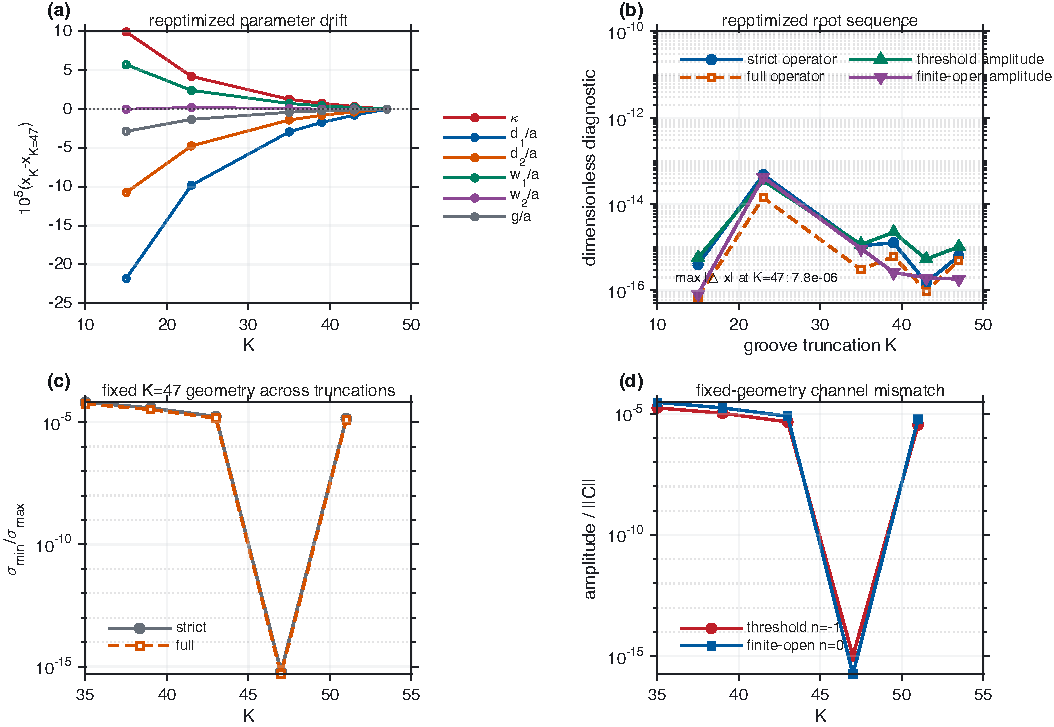
\includegraphics[width=\linewidth]{figures/figS1_extended_convergence.pdf}
\caption{\label{fig:s-convergence}
Detailed modal convergence.  (a) Reoptimized parameter drift relative to the
$(377,47)$ root.  (b) Strict/full residuals and unconstrained radiation
amplitudes at the reoptimized roots.  (c,d) Fixed highest-$K$ geometry
evaluated at neighboring truncations.  The latter panels are a discretization
crosscheck, not a failure of the independently reoptimized sequence.}
\end{figure*}

\section{Final-geometry complex-pole continuation}

The superseded pole cache used an intermediate $(121,15)$ root and is not used
in the revised figures.  The reported continuation starts from the final
$(313,39)$ geometry.  For target order $n=-1$, a local target normal
wavenumber $\bar q$ defines
\begin{equation}
 \Omega_p=\sqrt{(\kappa-1)^2+\bar q^2},\qquad
 Q=\frac{\Re\Omega_p}{2|\Im\Omega_p|}.                                 \label{eq:s-pole}
\end{equation}
Thirteen nonzero points span
$10^{-5}\leq|\Delta\kappa|\leq10^{-3}$, followed by the exact endpoint.
All accepted complex roots have singular-value ratio below $10^{-7}$; the
minimum consecutive mode overlap is $0.999999500$, and no branch jump is
detected.  Over $3\times10^{-5}\leq|\Delta\kappa|\leq10^{-3}$,
\begin{equation}
 \log Q=(-1.99590867)\log|\Delta\kappa|+\mathrm{const}.                 \label{eq:s-pole-fit}
\end{equation}
The nearest finite value is $Q=2.02613\times10^{12}$ at
$|\Delta\kappa|=10^{-5}$.  Equation~\eqref{eq:s-pole-fit} is a local
finite-model fit, not a universal Rayleigh-BIC exponent.

\section{Homogeneous-field construction}

All three main-text field maps use the same grid
$0\leq x/a\leq1$, $-0.75\leq y/a\leq1.05$ and the same color range.  Each
coefficient vector is normalized in Euclidean norm; the plotted pressure is
then divided by its maximum magnitude inside the grooves.  The strict BIC
coefficients are obtained at $(313,39)$ and truncated to $(121,15)$ only for
stable field sampling.  The other two fields are last right singular vectors
of the complete real-frequency homogeneous operator and are explicitly
surrogates rather than exact quasinormal modes.

\begin{table*}[t]
\caption{\label{tab:s-fields}Homogeneous-field diagnostics.  ``Exterior/groove''
is a finite-window normalized energy proxy, not an absolute modal energy.}
\begin{ruledtabular}
\begin{tabular}{ccccccc}
state & $\Omega$ & $\theta$ (deg) & $\sigma_{\mathrm{rel}}$ &
$|A_{-1}|/\|A\|$ & $|A_0|/\|A\|$ & exterior/groove\\
\hline
strict BIC & 0.916151303 & 5.25122 & $1.26\times10^{-15}$ & 0 & 0 & 0.0742\\
near-BIC surrogate & 0.915551303 & 5.25467 & $2.53\times10^{-3}$ & 0.0203 & 0.00262 & 0.0736\\
ordinary surrogate & 0.865500000 & 5.55947 & $1.31\times10^{-3}$ & 0.886 & 0.0697 & 0.752\\
\end{tabular}
\end{ruledtabular}
\end{table*}

For the strict state the exterior norm proxy reaches $0.017690$ by $H=a$ and
$0.017702$ by $H=5a$, remaining unchanged through $20a$.  Adding a nonzero
grazing component produces the expected linear term and increases the same
proxy to $0.067702$ at $20a$.

\section{Single-cavity ablation and two radiation phasors}

The single-cavity comparison is a declared numerical search, not a theorem.
It varies $x=(\kappa,d/a,w/a)$ over
\begin{align}
 0.04&\leq\kappa\leq0.25,\nonumber\\
 0.04&\leq d/a\leq2.00,\nonumber\\
 0.50&\leq w/a\leq0.95.                                              \label{eq:s-single-bounds}
\end{align}
at the exact $n=-1$ Rayleigh relation $\Omega=1-\kappa$.  A deterministic
1800-point survey and 14 bounded local refinements are followed through
$(N,K)=(221,44)$.  The best final point is
$(\kappa,d/a,w/a)=(0.04,0.520817128,0.530693214)$, with
$\sigma_{\mathrm{rel}}=0.1245882$, raw residual $1.48399$, and transverse
coefficient fraction $0.961$.  Extra transverse modes therefore do not close
both channels in this large rectangular-groove family.  The lower aperture
bound $w/a=0.50$ is part of the ablation definition; arbitrary narrow,
compound, or internally structured one-cavity designs are outside its scope.

For the two-groove mode, each radiation row can be decomposed as
\begin{equation}
 A_m^{\hom}=\sum_{\ell,q}\mathcal R_{m,\ell q}C_{\ell q},
 \qquad m=-1,0.                                                         \label{eq:s-phasor}
\end{equation}
The unnormalized two-groove sums are
$1.60\times10^{-16}$ for $n=-1$ and $1.06\times10^{-16}$ for $n=0$;
after normalization by the largest individual groove contribution, their
closures are $1.6\times10^{-15}$ and $1.1\times10^{-15}$.  This supports the
two-phase interpretation within the searched family.

\section{Dimensional scaling and sound-speed control}

With all normalized dimensions and $\theta$ fixed, set
$a=s a_0$.  The exact similarity law is
\begin{equation}
 f_{\mathrm{BIC}}(c,s)=\frac{\Omega_0c}{s a_0}
 =f_0\frac{c}{c_0}\frac{1}{s}.                                        \label{eq:s-similarity}
\end{equation}
The modal operator is rebuilt at every dimensional point.  For
$c=1400:10:1600$~m/s with $s=1$, $f_{\mathrm{BIC}}$ spans
$186.666667$--$213.333333$~kHz and the strict raw residual remains between
$9.69\times10^{-14}$ and $1.14\times10^{-13}$.  For
$s=0.5:0.1:2$ with $c=c_0$, the frequency spans $400$--$100$~kHz and the
raw residual remains between $9.16\times10^{-14}$ and
$1.86\times10^{-13}$.

As a control, the geometry, $f=200$~kHz, and $\theta$ are then held fixed
while $c$ changes.  Only $c=1500$~m/s remains at the Rayleigh threshold.  The
full-operator raw residual reaches $0.649$ and the open-amplitude ratio reaches
$0.776$ over the sweep.  The retuned similarity result must therefore not be
called temperature or environmental robustness of a fixed sample.

\begin{figure*}[t]
\centering
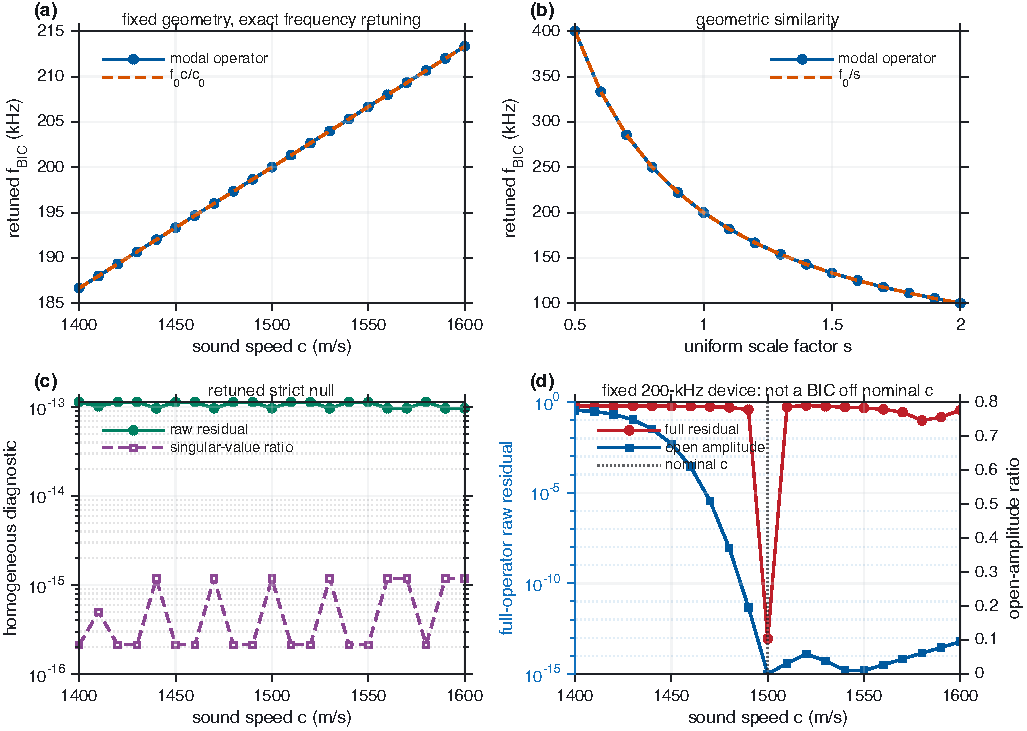
\includegraphics[width=\linewidth]{figures/figS2_scaling_environment.pdf}
\caption{\label{fig:s-scaling}
Dimensional similarity and fixed-device control.  (a) BIC frequency versus
sound speed under exact frequency retuning.  (b) Inverse scaling with uniform
geometric factor.  (c) Retuned homogeneous residuals remain at numerical
precision.  (d) At fixed geometry, frequency, and angle, changing sound speed
detunes the full operator and reopens radiation; off nominal $c$ these points
are not Rayleigh BICs.}
\end{figure*}

\section{Fabrication perturbations}

The fabrication ensemble keeps the final period, frequency, sound speed, and
Bloch point fixed and perturbs the five normalized dimensions.  For each
bound $p=1\%,2\%,5\%$:
\begin{itemize}
\item the ``one-parameter'' ensemble contains 100 balanced samples, cycling
through $d_1,d_2,w_1,w_2,g$ and drawing the selected error uniformly from
$[-p,p]$;
\item the ``joint'' ensemble contains 100 samples with all five errors drawn
independently and uniformly from $[-p,p]$.
\end{itemize}
The random seed is 260824 and the ensemble truncation is $(185,23)$.  All 600
geometries are valid and all solves finish.  The unperturbed final geometry at
this truncation has strict singular-value ratio $1.8210\times10^{-4}$ and raw
residual $2.2198\times10^{-3}$, which is recorded as the discretization floor.

The strict raw residual is evaluated after enforcing
$A_{-1}^{\hom}=A_0^{\hom}=0$.  In contrast, the threshold error reported below
is the physically informative unconstrained value
\begin{equation}
 \epsilon_{-1}=\frac{|A_{-1}|}{\|\bm A\|_2},\qquad
 \epsilon_0=\frac{|A_0|}{\|\bm A\|_2}.                                 \label{eq:s-tol-errors}
\end{equation}
The strict operator's target amplitude is exactly zero by construction and is
not used as a tolerance metric.

\begin{table*}[t]
\caption{\label{tab:s-tolerance}Five-parameter tolerance statistics.  Entries
are 5th/50th/95th percentiles.}
\begin{ruledtabular}
\begin{tabular}{cccc}
ensemble & bound & strict raw residual & unconstrained $\epsilon_{-1}$\\
\hline
one parameter & $\pm1\%$ & 0.00250 / 0.0136 / 0.429 & 0.000140 / 0.00315 / 0.214\\
one parameter & $\pm2\%$ & 0.00440 / 0.0359 / 0.611 & 0.000930 / 0.00784 / 0.432\\
one parameter & $\pm5\%$ & 0.0151 / 0.0696 / 0.591 & 0.00411 / 0.0194 / 0.809\\
joint five parameter & $\pm1\%$ & 0.0595 / 0.351 / 0.526 & 0.00951 / 0.162 / 0.273\\
joint five parameter & $\pm2\%$ & 0.183 / 0.580 / 0.842 & 0.0604 / 0.338 / 0.522\\
joint five parameter & $\pm5\%$ & 0.302 / 0.576 / 1.44 & 0.0866 / 0.637 / 0.948\\
\end{tabular}
\end{ruledtabular}
\end{table*}

\begin{figure*}[t]
\centering
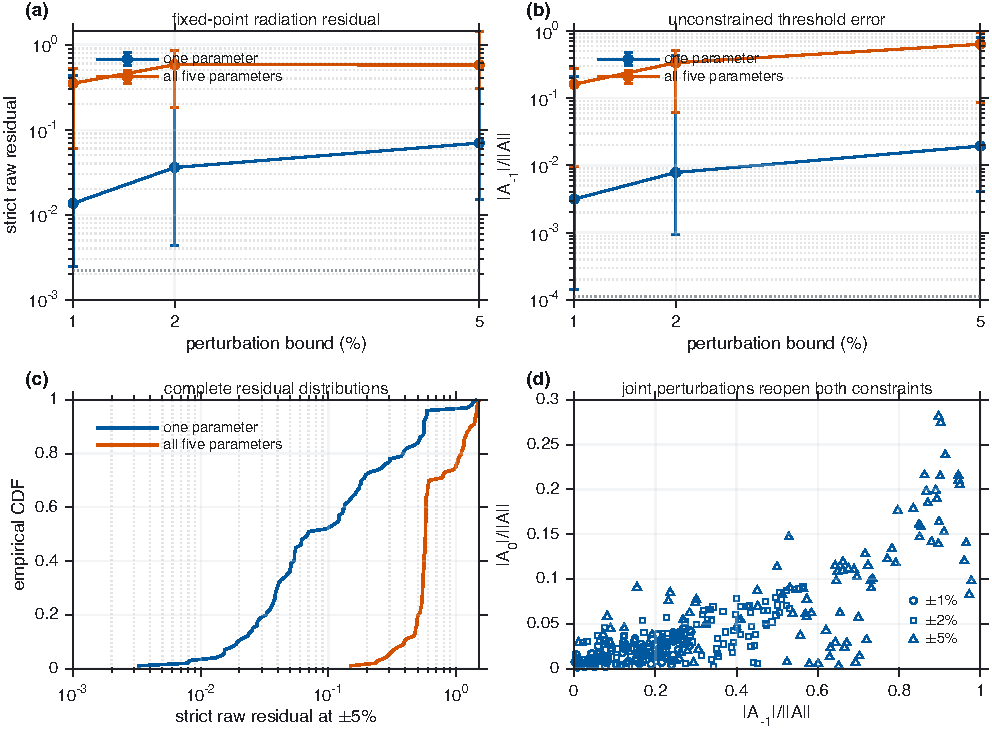
\includegraphics[width=\linewidth]{figures/figS3_tolerance_statistics.pdf}
\caption{\label{fig:s-tolerance}
Fabrication statistics at fixed Rayleigh point.  (a,b) Residual and
unconstrained threshold error; markers are medians and bars are 5--95\%
intervals.  (c) Full $\pm5\%$ residual distributions.  (d) Joint
perturbations reopen both the threshold and finite-flux amplitudes.  These
uniform local ensembles are sensitivity diagnostics, not a manufacturing
process model or yield prediction.}
\end{figure*}

\section{Driven scattering: reciprocal but not converged routing}

Driven scattering is not used to certify the homogeneous BIC.  It is included
to audit potential observables and to expose the truncation sensitivity of the
previous route point.  The final geometry is held fixed at
$f=200216.874212$~Hz and $\theta=+6^\circ$.  Direct solver results are listed
in Table~\ref{tab:s-route}; no cached efficiency table is used.

\begin{table*}[t]
\caption{\label{tab:s-route}Fixed-geometry driven route.  The target is
$n=-1$ for positive incidence.}
\begin{ruledtabular}
\begin{tabular}{ccccc}
$(N,K)$ & $\eta_{-1}$ & $\eta_0$ & condition number & energy error\\
\hline
$(81,11)$ & 0.00009184 & 0.9999082 & $1.95\times10^4$ & $1.1\times10^{-16}$\\
$(121,15)$ & 0.00040379 & 0.9995962 & $4.68\times10^4$ & $1.0\times10^{-15}$\\
$(201,25)$ & 0.00659293 & 0.9934071 & $2.61\times10^5$ & $1.3\times10^{-15}$\\
$(313,39)$ & 0.30606113 & 0.69393887 & $2.59\times10^6$ & $3.7\times10^{-14}$\\
$(401,50)$ & 0.05715278 & 0.94284722 & $1.41\times10^6$ & $3.2\times10^{-14}$\\
\end{tabular}
\end{ruledtabular}
\end{table*}

The efficiency is plainly nonconverged at fixed geometry and frequency.
Energy closure remains below $10^{-13}$, so the variation is not hidden power
loss; it is a truncation/conditioning problem.  At $(313,39)$, reversal to
$-6^\circ$ exchanges the signed target order:
\begin{align}
 \eta_{-1}(+6^\circ)&=0.306061126315,\nonumber\\
 \eta_{+1}(-6^\circ)&=0.306061126315.                                \label{eq:s-reciprocal}
\end{align}
with difference $1.10\times10^{-13}$.  The output angles are
$\mp80.336964^\circ$.  This is reciprocal signed-order exchange, not an
isolator or a converged one-way channel.

A separate ordinary point at $f=202430$~Hz and
$\theta=32.6328^\circ$ gives target efficiencies
$0.9779112$, $0.9929755$, $0.9986358$, $0.9996289$, $0.9999151$, and
$0.9996185$ for $(81,11)$ through $(401,50)$.  The final nonmonotonic step is
retained.  At $(401,50)$, $\eta_{-1}=0.9996185039$,
$\eta_0=0.0003814961$, condition number $7.32\times10^3$, and energy error
$8.9\times10^{-15}$.  Its active Rayleigh frequency is approximately
$141.825$~kHz; the state is therefore off Rayleigh and not BIC-enhanced.

\begin{figure*}[t]
\centering
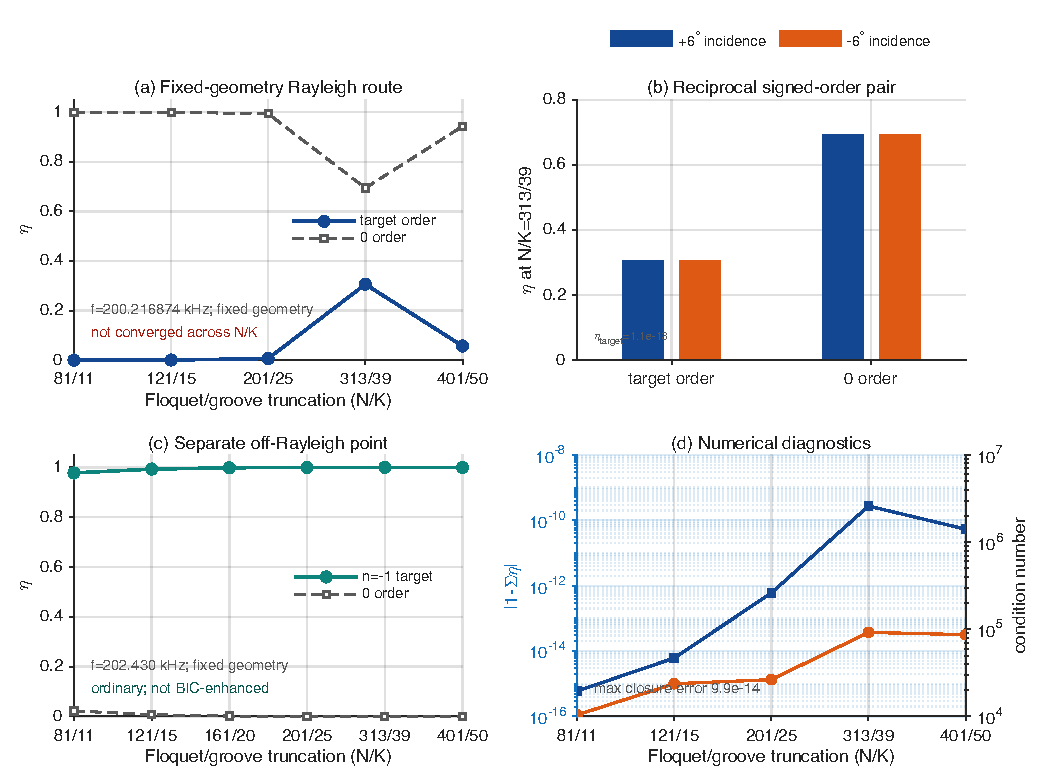
\includegraphics[width=\linewidth]{figures/figS4_driven_scattering.pdf}
\caption{\label{fig:s-driven}
Driven-scattering audit.  (a) Fixed-geometry route efficiency versus modal
truncation.  (b) Reciprocal signed-order pair at the illustrative $(313,39)$
point.  (c) Separate off-Rayleigh ordinary reflector.  (d) Energy-closure
error and matrix condition number for the route sweep.  Panel (a) precludes a
claim of converged device efficiency.}
\end{figure*}

\section{Proposed future water-tank validation}

No experiment is reported in the Letter.  Figure~\ref{fig:s-experiment}
records a falsifiable protocol for a later finite-sample study.  The proposed
sample set includes the full two-groove array, a flat rigid reference, a
single-large-cavity control, and the two-groove cell with the small cavity
blocked.  Several array lengths should be compared before interpreting a
linewidth as an infinite-period $Q$.

The water sound speed should be measured by time of flight.  The source
angular spectrum, complex hydrophone transfer function, and flat-plate
reflection should be calibrated.  Complex pressure can be sampled over
several periods at height $y_0$ and fitted as
\begin{align}
 p_{\mathrm{sc}}(x,y_0)
 &=\sum_n\widetilde A_n(y_0)\e^{-\ii k_{x,n}x},\nonumber\\
 A_n&=\widetilde A_n(y_0)\e^{+\ii k_{y,n}y_0}.                       \label{eq:s-field-fit}
\end{align}
The fitted amplitudes are then converted to normal-power efficiencies with
Eq.~\eqref{eq:s-eta}.  A grazing pressure feature must be reported separately
from its zero normal power.

For a narrowband burst, an amplitude ring-down
$p(t)\propto\exp(-t/\tau_A)$ would give
\begin{equation}
 Q_{\mathrm{ring}}=\pi f\tau_A.                                        \label{eq:s-ring}
\end{equation}
Finite width, source aperture, viscothermal attenuation, elastic backing,
and dimensional uncertainty must enter the comparison.  A driven reflection
minimum alone cannot validate Eq.~\eqref{eq:s-strict}.

\begin{figure*}[t]
\centering
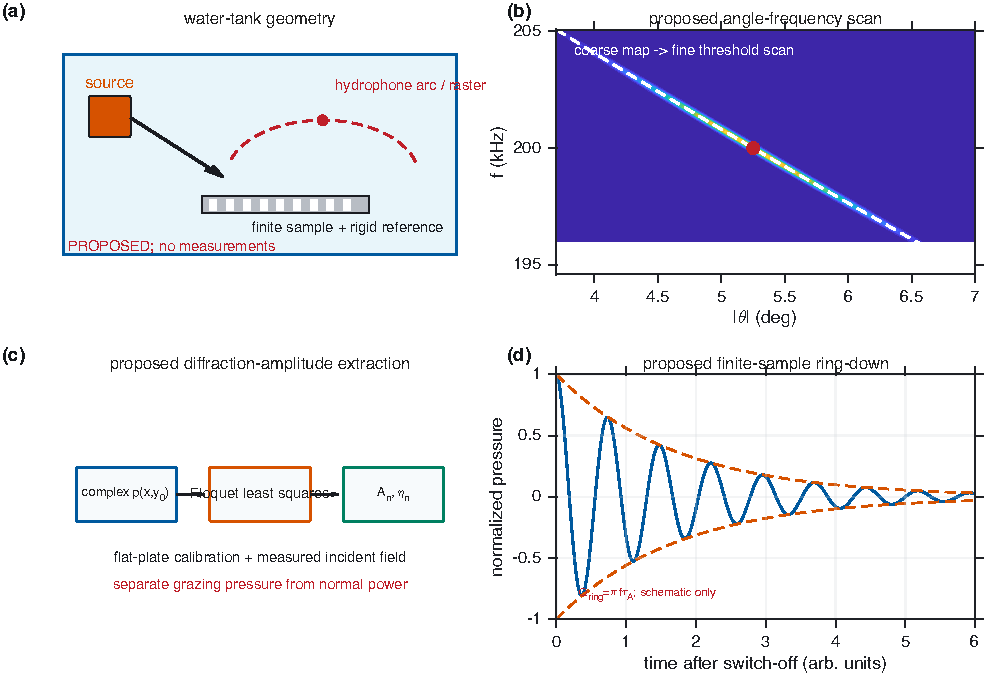
\includegraphics[width=\linewidth]{figures/figS5_proposed_experiment.pdf}
\caption{\label{fig:s-experiment}
PROPOSED future protocol; no measured data are shown.  (a) Water-tank geometry
with finite sample, flat reference, source, and hydrophone scan.  (b) Coarse
and fine angle-frequency scan around the threshold.  (c) Complex-field
Floquet extraction.  (d) Finite-sample ring-down schematic.}
\end{figure*}

\section{Data and code map}

The principal reproducible entry points are:
\begin{itemize}
\item \path{advanced_analysis/final_root_pole_validation.m};
\item \path{advanced_analysis/extended_convergence.m};
\item \path{advanced_analysis/scaling_environment.m};
\item \path{advanced_analysis/robustness_fields.m};
\item \path{advanced_analysis/driven_scattering_audit.m};
\item \path{advanced_analysis/run_prl_completion_figures.m}.
\end{itemize}
Machine-readable CSV/MAT outputs are stored in the corresponding
\path{advanced_analysis/} subdirectories.  The final design cache is
\path{Ni2019_MATLAB/results/StrictRayleighBIC_200kHz_min1mm.mat}.
The superseded intermediate pole cache and the previous hard-coded router
convergence table are not used in this revised evidence set.

\end{document}
